\section{Numerical ODEs}

Equations of the form \colorbox{shadecolor}{$y'(x)=f(x,y(x))$.}

\subsection{Explicit Euler Method}

Applying Taylor expansion with order $p=1$:
\begin{align*}
    y(x+h)=y(x)+y^{\prime}(x)h+{\frac{y^{(2)}(\xi)}{(2)!}}h^{2}
\end{align*}
\begin{align*}
    y(x+h) & = y(x)+f(x,y(x))h \\
    & + {\frac{1}{2!}}\left(
    \frac{\partial{f}(\xi,y(\xi))}{\partial x}1 + \frac{\partial f(\xi,y(\xi))}{\partial y}f(\xi,y(\xi))
    \right)h^{2}
\end{align*}

resulting in the following scheme:
\begin{align*}
    & y_0 = y(x_0) \\
    & y(x_0 + h) \approx y_1 = y_0 + f(x_0,y_0)h=y(x_0)+y'(x_0)h \\
    &\quad\vdots \\
    & \colorbox{shadecolor}{
        $y_{k+1} = y_k+f(x_k,y_k)h\quad(k=0,\ldots,n)$
    }
\end{align*}

with $h$ as step size (not necessarily constant).

\paragraph{Global Error} The global error is the maximum difference to the exact solution
\begin{align*}
    \colorbox{shadecolor}{$\displaystyle\max_{0\leq i\leq k}|y_i-y(x_i)|$}
\end{align*}

\emph{Convergence}: Global error $\to 0\text{ with }\max_i h_i\to 0$

\paragraph{Local Error} The local/step error is the error after one step from a correct starting point,
excluding past errors made:
\begin{snugshade*}
    \begin{align*}
        & \textbf{Slope error} : \underbrace{\tau_h(x_n) := \frac{y(x_n + h) - y(x_n)}{h}}_\text{True slope} -
            {\color{blue} \underbrace{(y'(x_n)=f)}_\text{approx. slope}} \\
        & \textbf{Output local error} : h\tau_h(x_n) := \underbrace{y(x_n+h)}_\text{True output} -
        \underbrace{(y(x_n)+{\color{blue}f}\cdot h)}_\text{Euler output}
    \end{align*}
\end{snugshade*}


For higher order slopes, the {\color{blue}approximate slope} is
\begin{align*}
    \frac{y'(x_n)}{1!}+\frac{y''(x_n)}{2!}h^1+\ldots+\frac{y^{(p)}(x_n)}{p!}h^{p-1}
\end{align*}

\emph{Consistency}: $\tau_h\to0$ for $\max_i h_i\to 0$

\subsubsection{Higher-Order Local Taylor Methods}

The explicit Euler method used order $p=1$.
We can expand to a scheme of order $p$:
\begin{align*}
    & y_0=y(x_0) \\
    & y_{k+1}=y_{k}+{\frac{y'_{k}}{1!}}h_{k}+{\frac{y''_k}{2!}}h_{k}^{2}+
    \frac{y'''_k}{3!}h_{k}^{3}+\cdots+{\frac{y_k^{(p)}}{p!}}h_{k}^{p}
\end{align*}

The local Taylor method is convergent with order $p$:
\begin{align*}
    \underbrace{\max_{0\leq i\leq k}|y_i-y(x_i)|}_\text{global error}=\mathcal{O}(h^p)\quad(h\to0)
\end{align*}
(simplified, with some constants $=\max_{0\leq i\leq k}h_i$).

However, they come with rather high costs arising from computing higher-order derivatives.

\subsection{Runge-Kutta Methods}

Designed to mimic the Taylor method, but without computing derivatives.
Instead, they use function evaluations at intermediate points.

\subsubsection{Explicit Midpoint/Heun Method of Order 2}

For the two-stage Runge-Kutta method, we have
\begin{align*}
    k_1 & = hf(x,y) \\
    k_2 & = hf(x+mh, y+mk_1) \\
    y(x+h) & = y(x) + ak_1 + bk_2
\end{align*}
using the ``traditional notation'' with h being a part of the function evaluation.

With constants $a=\frac{1}{2}, b=\frac{1}{2}$ and $m=1$, we have Heun's method:
\begin{align*}
    y_0 & = y(x_0) \\
    y_{k+1} & = y_k + \frac{h_k}{2}\left(f(x_k,y_k)+f(x_k+h_k,y_k+hf(x_k,y_k))\right)
\end{align*}

\subsubsection{Explicit ``Classical'' Runge-Kutta Method of Order 4}

Assuming that r.h.s.\ function $f$ has continuous partial derivatives up to order 4, we have
\begin{align*}
    k_1 & = hf(x,y) \\
    k_2 & = hf(x+\frac{1}{2}h, y+\frac{1}{2}k_1) \\
    k_3 & = hf(x+\frac{1}{2}h, y+\frac{1}{2}k_2) \\
    k_4 & = hf(x+h, y+k_3) \\
    y(x+h) & = y(x) + \frac{1}{6}(k_1+2k_2+2k_3+k_4)
\end{align*}

\subsubsection{General Framework (Butcher Tableau)}

\begin{snugshade*}
    A step from $x_n$ to $x_{n+1}=x_n+h_n\quad(n\in\mathbb{N})$ where ${\color{darkgreen}h_n}$ is the step size (variable or fixed)
    is given by
    \begin{align*}
        \left.
        \begin{matrix}
            k_{1}=f(x_n+{\color{blue}c_1}{\color{darkgreen}h_n},y_n+{\color{darkgreen}h_n}\sum_{j=1}^{s}{\color{purple}a_{1,j}}k_j) \\
            k_{2}=f(x_n+{\color{blue}c_2}{\color{darkgreen}h_n},y_n+{\color{darkgreen}h_n}\sum_{j=1}^{s}{\color{purple}a_{2,j}}k_j) \\
            \vdots                                                            \\
            k_{s}=f(x_n+{\color{blue}c_s}{\color{darkgreen}h_n},y_n+{\color{darkgreen}h_n}\sum_{j=1}^{s}{\color{purple}a_{s,j}}k_j)
        \end{matrix}
        \right\}
        \begin{array}{l}
            s \text{ stages, } \\
            {\color{gray} h\text{ not part of it}} \\
            {\color{gray} \text{(more general)}}
        \end{array}
    \end{align*}

    and the next step is
    \begin{align*}
        y_{n+1}=y_n+{\color{darkgreen}h_n}\sum_{j=1}^{s}{\color{red}b_j}k_j
    \end{align*}
\end{snugshade*}

the coefficients $a_{i,j},b_i,c_i$ are given in the Butcher tableau:

\begin{snugshade*}
    \begin{align*}
        \begin{array}{c|ccc}
            {\color{blue}c_1}    & {\color{purple}a_{1,1}} & {\color{purple}\cdots} & {\color{purple}a_{1,s}} \\
            {\color{blue}\vdots} & {\color{purple}\vdots}  & {\color{purple}\ddots} & {\color{purple}\vdots}  \\
            {\color{blue}c_s}    & {\color{purple}a_{s,1}} & {\color{purple}\cdots} & {\color{purple}a_{s,s}} \\
            \hline
            & {\color{red}b_1}     & {\color{red}\cdots} & {\color{red}b_s}
        \end{array}
    \end{align*}
\end{snugshade*}

for \textbf{explicit} methods, the tableau is \emph{lower triangular} (${\color{purple}a_{ij}} = 0\ (j \geq i)$):
\begin{align*}
    \begin{array}{c|cccc}
        {\color{blue}0}      & {\color{purple}0}       & {\color{purple}0}       & {\color{purple}\cdots} & {\color{purple}0}      \\
        {\color{blue}c_2}    & {\color{purple}a_{2,1}} & {\color{purple}0}       & {\color{purple}\cdots} & {\color{purple}0}      \\
        {\color{blue}\vdots} & {\color{purple}\vdots}  & {\color{purple}\ddots}  & {\color{purple}\ddots} & {\color{purple}\vdots} \\
        {\color{blue}c_s}    & {\color{purple}a_{s,1}} & {\color{purple}a_{s,2}} & {\color{purple}\cdots} & {\color{purple}0}      \\
        \hline
        & {\color{red}b_1}     & {\color{red}b_2}     & {\color{red}\cdots} & {\color{red}b_s}
    \end{array}
\end{align*}

and has to satisfy the row-sum property $c_i = \sum_{j=1}^{s}a_{i,j} = \sum_{j=1}^{i-1}a_{i,j}\ (i=2,\ldots,s)$
(for ``simulation'' of Taylor method).

The \textbf{local error} of a step is
\begin{align*}
    \tau_{h}(x_{n}) := \frac{y(x_{n}+h)-y(x_{n})}{h}-\left(\sum_{j=1}^{s}b_{j}k_{j}\right)
\end{align*}

some common butcher tableaus for explicit methods are:

\makebox[\columnwidth]{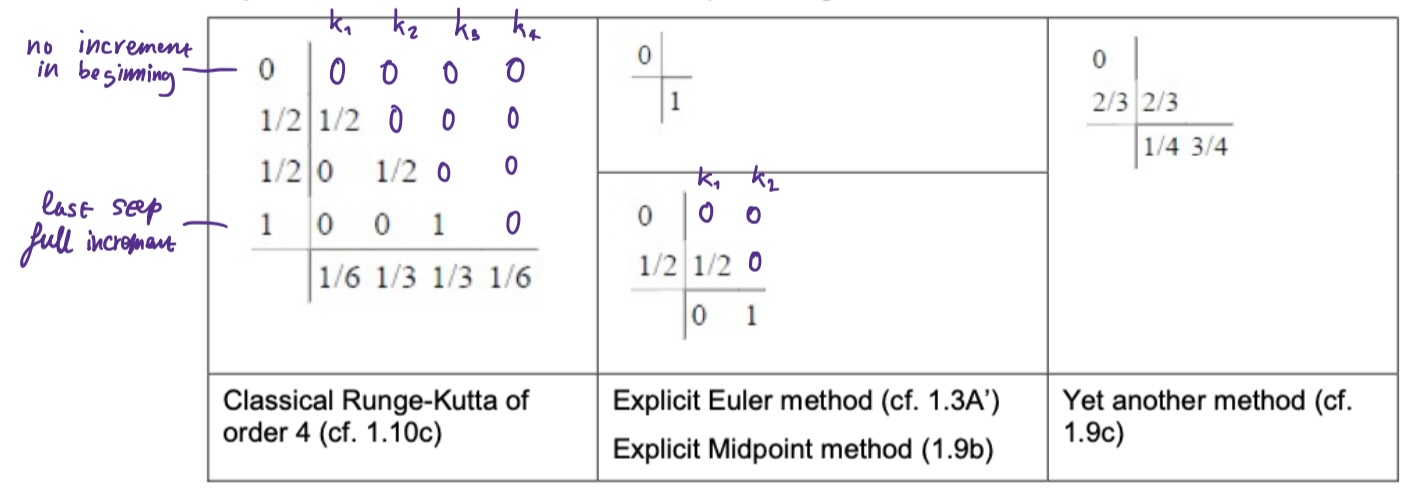
\includegraphics[width=\columnwidth]{images/butcher_tableau}}

\subsection{Adaptive Explicit Runge-Kutta Methods}
